
%----------------------------------------------------------------------------------------
%	PACKAGES AND OTHER DOCUMENT CONFIGURATIONS
%----------------------------------------------------------------------------------------

\documentclass[paper=a4, fontsize=11pt]{scrartcl} % A4 paper and 11pt font size

\usepackage[utf8]{inputenc}
\usepackage[T1]{fontenc} % Use 8-bit encoding that has 256 glyphs
\usepackage[polish]{babel} % English language/hyphenation
\usepackage{amsmath,amsfonts,amsthm} % Math packages

\usepackage{babelbib}

\usepackage{graphicx}
\usepackage{sectsty} % Allows customizing section commands
%\allsectionsfont{\centering \normalfont\scshape} % Make all sections centered, the default font and small caps
\usepackage{hyperref}

\usepackage{fancyhdr} % Custom headers and footers
\pagestyle{fancyplain} % Makes all pages in the document conform to the custom headers and footers
\fancyhead{} % No page header - if you want one, create it in the same way as the footers below
\fancyfoot[L]{} % Empty left footer
\fancyfoot[C]{} % Empty center footer
\fancyfoot[R]{\thepage} % Page numbering for right footer
\renewcommand{\headrulewidth}{0pt} % Remove header underlines
\renewcommand{\footrulewidth}{0pt} % Remove footer underlines
\setlength{\headheight}{13.6pt} % Customize the height of the header

\numberwithin{equation}{section} % Number equations within sections (i.e. 1.1, 1.2, 2.1, 2.2 instead of 1, 2, 3, 4)
\numberwithin{figure}{section} % Number figures within sections (i.e. 1.1, 1.2, 2.1, 2.2 instead of 1, 2, 3, 4)
\numberwithin{table}{section} % Number tables within sections (i.e. 1.1, 1.2, 2.1, 2.2 instead of 1, 2, 3, 4)

\setlength\parindent{0pt} % Removes all indentation from paragraphs - comment this line for an assignment with lots of text

%----------------------------------------------------------------------------------------
%	TITLE SECTION
%----------------------------------------------------------------------------------------

\newcommand{\horrule}[1]{\rule{\linewidth}{#1}} % Create horizontal rule command with 1 argument of height

\title{	
\normalfont \normalsize 
\textsc{Grafy i sieci} \\ [25pt] % Your university, school and/or department name(s)
\horrule{0.5pt} \\[0.4cm] % Thin top horizontal rule
\huge SK2. Wizualizacja algorytmów grafowych II \\ % The assignment title
\horrule{2pt} \\[0.5cm] % Thick bottom horizontal rule
\LARGE Dokumentacja końcowa
}%


\author{Michał Kielak, Michał Uziak} % Your name

\date{\normalsize\today} % Today's date or a custom date

\begin{document}

\maketitle % Print the title

%----------------------------------------------------------------------------------------
%	PROBLEM 1
%----------------------------------------------------------------------------------------

\section{Cel projektu}

Celem projektu jest implementacja oprogramowania do wizualizacji wybranych algorytmów kolorowania grafu.

\section{Algorytm}

W projekcie zostanie użyty algorytm Kruskala, wyznaczający minimalne drzewo rozpinające dla spójnego, ważonego grafu nieskierowanego. Algorytm został stworzony przez Josepha Kruskala w 1956 roku.
 

\subsection{Opis działania algorytmu Kruskala}

Kroki tworzenia drzewa w algorytmie Kruskala:
\begin{itemize}
	\item utworzenie lasu z wierzchołków (każdy wierzchołek jest osobnym drzewem) - zbiór L
	\item posortowanie krawędzi wg wag - zbiór S
	\item dopóki S>0
		\begin{itemize}
			\item wybranie i usunięcie krawędzi o najmniejszej wadze ze zbioru S
			\item jeśli krawędź łączyła dwa różne drzewa, dodanie jej do lasu L
			\item jeśli krawędź nie łączyła dwóch różnych drzew, usunięcie
		\end{itemize}
\end{itemize} 

\subsection{Złożoność obliczeniowa}

Poszczególne fazy algorytmu mają złożoności równe:
\begin{itemize}
	\item sortowanie krawędzi według wag - złożoność O(ElogV)
	\item tworzenie drzewa - O(E $\alpha$(E,V))
\end{itemize}
Zatem całkowita złożoność algorytmu wynosi O(ElogV) \\ \\
gdzie: \\ E - liczba punktów \\
V - liczba krawędzi \\
$\alpha$ - odwrotność funkcji Ackermanna


\section{Implementacja}

Projekt zostanie wykonany w języku Python, przy użyciu biblioteki Qt4. Założeniem programu jest działanie w czasie rzczywistym - użytkownik wprowadza przykładowy graf, następnie przechodząc przez kolejne etapy może prześledzić kroki tworzenia minimalnego drzewa rozpinającego. Algorytm kończy działanie, gdy wyznaczy minimalne drzewo rozpinające.
Przejście między kolejnymi krokami budowania drzewa będzie dla użytkownika niezauważalny, dlatego  czas wykonania algorytmu może zostać pominięty.

\subsection{Struktury danych}

Główną strukturą danych wykorzystywaną w projekcie będzie Graph z modułu networkx przeznaczonego dla grafów i sieci.

\subsection{Format wejścia i wyjścia}

Użytkownik będzie miał możliwość wprowadzenia danych na dwa sposoby:

\begin{itemize}
\item przez graficzny interfejs użytkownika (rysowanie punktów, krawędzi, podawanie wag)
\item przez wczytanie plików tekstowych
\end{itemize}

Format pliku wejściowego:

\begin{center}
MACIERZ WAG \\

1 1 1 0 \\
3 4 2 1 \\

WSPÓŁRZĘDNE WIERZCHOŁKÓW \\
x y z \\
x y z
\end{center}

Po wykonaniu programu, użytkownik będzie miał możliwość zapisania otrzymanego grafu w postaci pliku graficznego.

\subsection{Sytuacje wyjątkowe}   

Możliwe sytuacje wyjątkowe:
\begin{itemize}
\item wczytanie źle sformatowanego pliku - pojawienie się okna z informacją o błędzie
\item połączenie dwóch tych samych wierzchołków więcej niż jedną krawędzia - zignorowane, wybranie pierwszej ze zdefiniowanych krawędzie
\item osierocone wierzchołki - usunięcie zbędnych wierzchołków
\end{itemize}

\subsection{Dodatkowe opcje}   

\begin{itemize}
\item kolorowanie krawędzi
\item ustawianie wielkości punktów
\item zapisywanie, jako pliki graficzne, kolejnych kroków tworzenia drzewa
\end{itemize}

\section{Program - sposób obsługi}

\subsection{Okno główne}

Po uruchomieniu programu, pojawia się główne okno, które pokazano poniżej. Składowe okna głównego:
\begin{itemize}
\item[1] Menu (File)
\item[2] Pasek funkcji
\item[3] Plansza do rysowania i przetwarzania grafu
\end{itemize}

\begin{center}
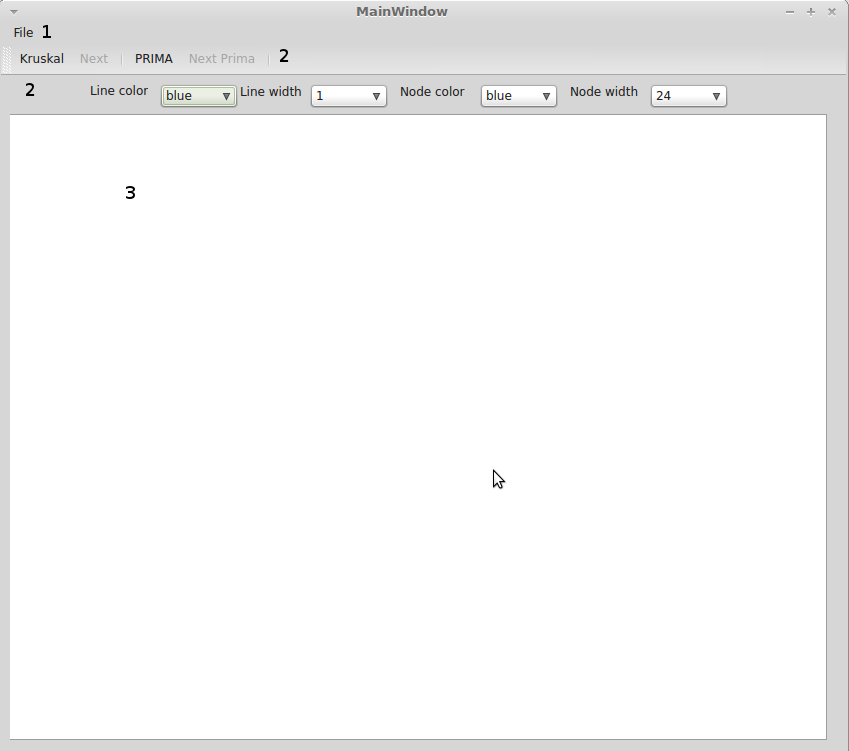
\includegraphics[width=12cm]{main_window.png}

\end{center}
\subsection{Menu główne}

Menu składa się z poniższych funkcji:
\begin{itemize}
\item Export nodes - zapisuje współrzędne dodanych punktów do pliku
\item Export weights - zapisuje krawędzie i wagi do pliku
\item Import nodes - wczytuje współrzędne punktów z pliku
\item Import weights - wczytuje krawędzie i wagi z pliku
\item Save to image file - zapisuje obraz widoczny w oknie rysowania do pliku graficznego
\end{itemize}

Uwaga! Wczytywanie zapisanego grafu powinno odbywać się w poniższej w kolejności:
\begin{itemize}
\item punkty
\item krawędzie i wagi
\end{itemize}

\subsection{Rysowanie grafu}
Do planszy można dodać dwa rodzaje obiektów:
\begin{itemize}
\item punkty
\item krawędzie pomiędzy punktami
\end{itemize}

Punkty dodaje się przez kliknięcie lewym przyciskiem myszy w dowolnym miejscu planszy. W wyniku kliknięcia pojawi się punkt.
Łączenie punktów krawędziami odbywa się w następujący sposób:
\begin{itemize}
\item kliknięcie w wybrany punkt początkowy
\item przytrzymanie przycisku
\item przeciągnięcie kursora myszy nad punkt końcowy, z którym ma być połączony punkt początkowy
\item puszczenie klawisza myszy
\end{itemize}

W wyniku wykonania powyższych operacji, pomiędzy punktami pojawi się krawędź z etykietą wagi. Podana waga odpowiada długości odcinka.

Przed narysowaniem obiektu, możliwa jest zmiana jego właściwości (za pomocą list rozwijanych na górze ekranu).
Dla linii są to:
\begin{itemize}
\item grubość linii (line width)
\item kolor linii (line color)
\end{itemize}

Dla punktu są to:
\begin{itemize}
\item średnica punktu (node width)
\item kolor punktu (node color)
\end{itemize}

\subsection{Wykonanie algorytmu}

Po narysowaniu grafu, możliwe jest wybranie jednego z dwóch algorytmów znalezienia minimalnego drzewa rozpinającego:
\begin{itemize}
\item Algorytm Kruskala
\item Algorytm PRIMA
\end{itemize}

Wyboru dokonuje się przez wciśnięcie wybranego przycisku u góry ekranu (odpowiednio "Kruskal" lub "Prima"). Następnie można obejrzeć kolejne kroki wykonania wybranego algorytmu, przez wciskanie przycisku "Next". Po zakończeniu wykonania algorytmu przycisk ulega dezaktywacji.

Podczas wykonywania algorytmu Kruskala dostępne jest okno, w którym widać posortowane wagi krawędzi. Wybierane w kolejnych krokach krawędzie są zaznaczane kolorem czerwonym.

\end{document}